\documentclass{interim}
\usepackage{physics, amssymb, graphicx, fancyvrb}
\usepackage[colorlinks=true, allcolors=blue]{hyperref}
\usepackage{pdfpages, multirow}
\usepackage{float}

% alternative font if you prefer
% \usepackage{times}

% for alternative page numbering use the following package
% and see documentation for commands
%\usepackage{fancyheadings}


% other potentially useful packages
% \uspackage{amssymb,amsmath}
% \usepackage{url}
% \usepackage{fancyvrb}
% \usepackage[final]{pdfpages}

\begin{document}

%%%%%%%%%%%%%%%%%%%%%%%%%%%%%%%%%%%%%%%%%%%%%%%%%%%%%%%%%%%%%%%%%%%
\title{3D Face Recognition from RGB Camera and Radar Sensor}
\author{Stergious Aji}
\date{\today}
\maketitle
%%%%%%%%%%%%%%%%%%%%%%%%%%%%%%%%%%%%%%%%%%%%%%%%%%%%%%%%%%%%%%%%%%%

%%%%%%%%%%%%%%%%%%%%%%%%%%%%%%%%%%%%%%%%%%%%%%%%%%%%%%%%%%%%%%%%%%%
{\hypersetup{hidelinks}\tableofcontents}
\newpage
%%%%%%%%%%%%%%%%%%%%%%%%%%%%%%%%%%%%%%%%%%%%%%%%%%%%%%%%%%%%%%%%%%%

%%%%%%%%%%%%%%%%%%%%%%%%%%%%%%%%%%%%%%%%%%%%%%%%%%%%%%%%%%%%%%%%%%%
\section{Introduction}\label{intro}
% briefly explain the context of the project problem
% Please note your proposal need not follow the included section headings - this is only a suggested structure. Also add subsections etc as required
% example references: \cite{BK08}

\subsection{Motivation}
Facial recognition technology is a key area of research within the field of computer vision, with widespread applications across areas such as security surveillance, forensic analysis, and human-computer interaction. Its most prominent use case lies in biometric authentication, allowing individuals access to their personal devices or restricted areas. This enables a non-invasive, hands-free approach to identity verification, removing the need to recall passwords. Furthermore, facial biometrics are naturally more accessible than other forms such as fingerprints, iris, or palm prints \cite{zhou20183d}.

Since its inception in the 1960s, facial recognition systems have evolved drastically. The pioneering work by Bledsoe \cite{bledsoe1966model} first distinguished faces by comparing distances of manually annotated landmark features such as the nose, eyes, and mouth. In more recent years, the advent of deep learning has enhanced the performance and efficiency of human face classification, benefitting from the vast online repositories of face images.  Nevertheless, these systems primarily rely on images captured by RGB cameras, making them susceptible to variations in lighting and pose \cite{xu2004depth}. By incorporating depth data, which draws attention to the geometric details of the face alone, the effect of such environmental factors can be mitigated. Moreover, the transition to three-dimensional face recognition not only improves accuracy, but also enhances the security of biometric systems against spoofing \cite{wen2015face}.

The popularity of 3D face recognition is on the rise, evidenced by its adoption in smartphones with the likes of Apple and their Face ID \cite{apple-faceid} technology. This growing demand has pushed the commercialisation of depth-sensing technology to smaller form factors, enabling it to operate efficiently, in real-time, on mobile devices with minimal computational power \cite{soumya2023recent}. Depth cameras used in this context typically employ an active face acquisition method. This is where non-visible light is projected onto the face and reflected back, allowing sensors to measure and map facial features. The most common approach involves lidar cameras, emitting waves in the near-infrared spectrum, due to their ability to capture a dense 3D map of the subject's face \cite{wang2020evolution}. However, its weakness in penetrating materials such as clothing and hair is a notable limitation. In contrast, millimetre radar waves (mmWaves) can penetrate such obstacles to directly reach the dermal layer of the skin \cite{vizard2006advances}, potentially offering better performance in occlusion scenarios or even within the presence of rain or fog.

Research into the efficacy of radar waves for 3D face recognition is relatively sparse but recent studies show positive results \cite{hof2020face, lim2020dnn,kim2020face, pho2021radar,challa2021face}, further discussed in Section \ref{background:prior_work}. Radar technology is generally more cost-effective, both in terms of acquisition and computationally speaking, as it consumes less power in comparison to the more widely used lidar cameras. However, the lower accuracy and sparsity of millimetre wave signatures may hinder its effectiveness in facial recognition. A possible solution is to integrate the RGB information with depth data, obtained by radar sensors, to enhance the system's ability to accurately learn and identify facial characteristics.


\subsection{Aims}
This project aims to explore the effectiveness of using RGB cameras in conjunction with mmWave radar sensors for 3D facial recognition. Since there are no appropriate datasets available for this purpose, we will be required to collate this data ourselves. We plan to use the Intel RealSense L515 camera \cite{intel-l515} for capturing RGB images of an individual's face. Meanwhile, the Google Soli radar sensor \cite{lien2016soli} will be employed to gather depth information through reflected millimetre waves.

Given the necessity of data collection, our goal is to gather facial data from approximately 50 participants. This number is expected to be sufficient for both training and evaluating our proposed model within the limited timeframe. We aim to obtain face data under various conditions including diverse poses, lighting environments, and common occlusion scenarios. The objective is to empirically validate the benefits of utilising mmWave technology in this context. We hypothesise that this approach would yield a system that is invariant to pose, lighting, and occlusion compared to using RGB or depth information alone.

Next, we plan to develop a novel face recognition model using a deep Convolutional Neural Network. This model will be trained on the captured data in order to learn facial features from both the RGB and depth characteristics acquired from the Soli sensor. We also intend to investigate different techniques in fusing these two modalities, aiming to pinpoint the most effective strategy that provides rich and distinctive representations, for accurate face classification performance. The model's effectiveness will be benchmarked against prior radar-based facial recognition systems, as well as, a comparison to solely using RGB data.

% This RealSense camera also includes a LiDAR sensor which produces a more accurate dense depth image. As a backup, a separate model can be trained to transform the sparse Soli data into a more dense representation before inputting into the facial recognition model. However, if the radar data works well this may not be needed. (MAY NOT INCLUDE)

%%%%%%%%%%%%%%%%%%%%%%%%%%%%%%%%%%%%%%%%%%%%%%%%%%%%%%%%%%%%%%%%%%%
% \section{Statement of Problem??}

% clearly state the problem to be addressed in your forthcoming project. Explain why it would be worthwhile to solve this problem.

%%%%%%%%%%%%%%%%%%%%%%%%%%%%%%%%%%%%%%%%%%%%%%%%%%%%%%%%%%%%%%%%%%%
\section{Background Survey}
% present an overview of relevant previous work including articles, books, and existing software products. Critically evaluate the strengths and weaknesses of the previous work.
A review of the relevant literature in the field is undertaken and summarised in the following chapter. This is essential in corroborating best practices and gaining a deeper insight into the strengths and limitations of mmWave radar, within the context of face recognition. A look into existing databases compatible with our research objectives is then performed, followed by a detailed justification for the need to compile our own dataset. Furthermore, a critical analysis of the recent work studying radar-based human face classification is provided. Finally, an outline of multimodal data fusion techniques and deep learning architectures for face recognition will be laid out.

\subsection{mmWave Radar Technology}
Radio Detection and Ranging, or Radar, has been around for decades and is instrumental in fields such as space exploration, military and commercial aviation, maritime navigation, as well as, meteorology. Recently, the miniaturisation of radar sensors to the millimetre wave (mmWave) band has brought its application to more small-scale domains \cite{soumya2023recent}. A notable example is Google's integration of the Soli sensor into their Pixel 4 smartphones for facial detection and motion gesture recognition \cite{googleblog2020}. This is the exact sensor we plan to utilise during this project's data collection phase. A key driving factor for this choice is the Soli's use of Frequency Modulated Continuous Wave (FMCW) technology. This is proven to offer superior range resolution in comparison to other modulation techniques due to its high pulse compression \cite{mahafza2005radar}, a vital aspect for generating accurate facial embeddings. 

mmWave sensing is also being explored in the domain of autonomous vehicles, specifically in systems such as collision warnings and adaptive cruise control \cite{dfrobot}. This is primarily due to its edge over traditional near-infrared waves employed by Light Detection and Ranging (Lidar) cameras, particularly in its resilience to atmospheric conditions such as dust, smoke, fog, and rain \cite{cadenceblog2022}. This penetrative power of mmWaves make it a promising candidate for reliable facial recognition in evolving, real-world scenarios. However, it is important to note the trade-off, as mmWaves tend to have a lower accuracy in comparison. This could impact face recognition performance where precision in detecting and mapping facial features is paramount. This project will therefore explore counter-balancing this limitation with the information gained from RGB images, potentially paving the way for more resilient and versatile systems.


\subsection{Data Acquisition}
\label{background:data_acquisition}
Various techniques exist for capturing 3D face data which can be broadly categorised into two main types: \textit{Active} and \textit{Passive} systems \cite{zhou20183d}. Active systems emit non-visible light onto the target and use the reflected light to construct a 3D point cloud of the subject. Contrastingly, passive systems rely on the available light in the scene to capture facial features. For instance, stereoscopic cameras use two or more lenses to photograph the subject from different perspectives, enabling depth perception. 3D facial features can also be inferred using shape-from-shading techniques which analyse the luminance values contained within grayscale images \cite{horn1977understanding}.

Passive systems, advantageous for their ability to operate in real-time without light emission, are highly influenced by environmental lighting conditions. In contrast, active systems are more robust as they use their own light to illuminate the subject, permitting functionality even in dimly lit settings. Active acquisition often involves structured light and triangulation methods to gather depth information. In the case of lidar cameras like the Intel RealSense, the time-of-flight of emitted light is measured to gauge the distances of points on the target. The Soli sensor represents another active system, featuring a single transmit and three receiver antennas. The system measures the phase difference and Doppler shift of reflected mmWaves to estimate the distance and radial velocity of the target, respectively. 

When collecting data on human faces for 3D face recognition, it is crucial to ensure the data comprises a wide range of facial poses, expressions, lighting and occluding scenarios. The pure geometric information within 3D face scans, unlike standard images, allows for the training of models to be insensitive to such variations in the data. Research by Prabhu et al. \cite{prabhu2011unconstrained} found that the maximum pose angle that their Local Binary Pattern-based model is robust against is $60^\circ$. For this reason, the poses we capture will not exceed this angle since our goal is not to investigate extreme pose invariance, but instead the capabilities of radar waves for face recognition. Furthermore, a diverse range of genders, ages, and ethnicities are essential to generalise the model for real-world applications.

In recent years, the number of 3D face databases available has grown, encompassing various acquisition techniques and devices. Noteworthy datasets include the BU-3DFE \cite{yin20063d} and the FRGC \cite{phillips2005overview}, widely accepted as standard references for evaluating the performance of 3D face recognition systems. The BU-3DFE dataset, for example, focuses on facial expressions, containing six distinct types for each of the 100 individuals captured, using stereo photography. While these datasets are unsuitable for our project, the data collection procedure used to amass them provide valuable insights. Presently, there is only one public database featuring radar signatures of 206 human faces, available through an IEEE data port \cite{mmwavefacedata}. This dataset was obtained using a Qualcomm 60 GHz mmWave radar, but it lacks any RGB face images of the participants involved in the study. These factors motivate building our own dataset including both RGB images and mmWave face signatures of subjects. Such an approach affords us the flexibility in tailoring our experiment design to investigate the model's effectiveness under specific conditions, all while adhering to established data collection protocols.


\subsection{Prior Work on Radar-based Face Recognition}
\label{background:prior_work}
The use of millimetre waves for face identification is a relatively new research field, spurred by the commercialisation of radar sensor technology. One of the earliest studies found to investigate human identification using mmWaves can be traced back to 2019, conducted by Zhao et al. \cite{zhao2019mid}. Although this paper focuses on classifying subjects by their gait and body shape rather than facial features, it demonstrates the ability of mmWaves to encapsulate the subtle idiosyncrasies among individuals. These nuanced differences are vital for learning models to effectively differentiate between unique subjects, leading to high classification accuracies.

Following this, Hof et al. \cite{hof2020face} proposes a Deep Neural Network (DNN) based Autoencoder that can distinguish human faces captured by an 802.11ad/y networking chipset operating at a centre frequency of 60 GHz. The Autoencoder is able to encode mmWave face signatures of over 200 individuals with enough separation to distinguish between positive and negative instances by measuring their Mean Squared Error (MSE) against reference facial embeddings. The study conducted an extensive data collection process, capturing face scans of 206 participants comprising various genders and ages, in five different poses: frontal, as well as, $15^\circ$ and $25^\circ$ head rotations to the left and right. This collection was subsequently made available through an IEEE Data Port \cite{mmwavefacedata}. While this dataset encapsulates faces from a wide range of people, including some with beards and spectacles, it lacks representation of other common occlusion scenarios like head accessories, that our project aims to explore. Moreover, the study utilised a larger sensor containing a total of 1024 transmit and receiver antenna pairs, found to capture redundant information. This is in contrast to the compact Soli chip with a single transmit and three receiver antennas, intended to work within a smartphone. The study simulated the effect of reducing the antenna count to 10, markedly decreasing the distinctiveness of facial signatures. Promisingly, increasing the number of neurons in their Neural Network and an additional hidden layer could compensate for this reduction, maintaining high accuracy.

Lim et al. \cite{lim2020dnn} proposes another Deep Neural Network model, however with a more traditional Multi-Layer Perceptron (MLP) architecture where every layer is fully connected to adjacent ones. The study utilised a small-scale, 61 GHz FMCW radar sensor developed by bitsensing Inc. \cite{bitsensing2020bts60}, comparable to the Google Soli with a single transmit and three receiver antennas. The model attained a mean classification accuracy of 92\% across eight subjects, surpassing the performance of both, a Support Vector Machine (SVM), and a tree-based Ensemble Learning approach trained on the same face signatures. It is important to note the relatively small-sized dataset used to train the model, raising concerns about potential overfitting as the data is not representative enough. The paper provides limited details on the data collection methodology used, only mentioning that the facial distances ranged from 30 cm to 50 cm. It can be assumed then that the study likely focussed on frontal poses without any occlusions for all eight subjects. The research also explored the impact of using a single receiving antenna, which resulted in a reduced accuracy of 73.7\%. This finding is in line with Hof et al.'s \cite{hof2020face} observation that an increased number of receiving antennas can enhance classification accuracy by the ability to capture more nuanced facial features. The paper also suggests that a CNN may be more appropriate if signals were stacked on the time axis rather than the frequency axis.

During the same period, Kim et al. \cite{kim2020face} conducted research using an identical 61 GHz FMCW radar sensor from bitsensing Inc., featuring a range resolution of 2.5 cm. Their study introduces a CNN model comprising three convolutional layers and three fully connected layers. The radar data underwent heavy preprocessing to transform it into a more image-like format suitable for the CNN model. With a data split of 70\%/15\%/15\% for training, validation, and testing, the model achieved an average classification accuracy of 98.7\% on a limited dataset of only three individuals. Interestingly, the study also examined the impact of wearing cotton masks. The results showed a minimal drop in average classification accuracy by 0.9\%, which is encouraging for the objectives of our project. However, these findings are to be taken with caution due to the small size of the dataset. It remains unclear whether this level of performance would hold consistently across a larger and more diverse group of subjects, with more varied occlusions.

Pho et al. \cite{pho2021radar} adopts a One-Shot Learning approach to the problem. This is where the model is trained with a single or only a few labelled instances, beneficial when there is a lack of training samples available. The proposed method constitutes a Siamese structure of two identical CNNs with shared parameters that map the input radar signals into a latent space. A distance metric between the outputs of both CNNs is used during the training and testing phases to measure the similarity between face inputs. The model is specifically trained for \textit{binary classification} by inputting pairs of face signatures from either the same or different people. This process resulted in the model learning embeddings that push different faces into distinct Euclidean regions of the embedding space. The same bitsensing Inc. BTS60 chipset, used by Lim et al. and Kim et al. \cite{lim2020dnn, kim2020face}, is employed to capture 500 frames of the faces of eight participants. An average classification of 97.6\% was achieved, an improvement over the previous DNN model by Lim et al. involving the same number of people. t-Stochastic Neighbour Embedding (t-SNE) \cite{van2008visualizing} is then applied for dimensionality reduction. The resulting visualisations demonstrated that the one-shot Siamese network effectively separated each individual's face into exclusive regions, simplifying the classification task. Although a small dataset is used,\,only encompassing frontal poses with no occlusion\,settings, the proposed method is well documented and is likely robust against larger datasets.

Challa et al. \cite{challa2021face} employs two different machine learning models on the dataset made available through the IEEE port \cite{mmwavefacedata}. Their approach began with CNN-based Autoencoders followed by a Random Forest Ensemble Learning approach. A total of nine Autoencoders are built, each tailored to different frame rates, focusing on compressing and learning to reconstruct the original data from its compressed, latent form. The Autoencoders are trained using randomly selected data samples from a subset of 186 mmWave face signatures. The flattened and labelled outputs are then used to train and test nine discrete Random Forest models using identical hyperparameters, as recommended by the Sci-kit library. This methodology yielded impressive results, achieving an average classification accuracy of 99.98\% using all 1400 frames per individual. Even reducing the number of frames to 70 per person, the model was able to maintain a high accuracy of 97.1\%. The paper presents an approach that is unique in comparison to the rest of the research papers tackling this subject, showcasing an efficient model that is able to be deployed on mobile chips.

The research in this area exclusively focuses on utilising data from radar sensors, largely driven by concerns of privacy preservation. However, a significant limitation of this approach is the required duration for capturing an accurate facial scan. The sensor needs to operate for several seconds, typically in the range between 10 and 15 seconds, in order to obtain a detailed scan. Such a time frame is impractical in real-world situations, as it necessitates the subject to remain motionless for a prolonged period. Up to this point, no study was found to explore the potential benefits of combining radar signatures with corresponding RGB data to enhance facial recognition capabilities. Given the high performance of existing deep learning models using RGB images alone, such as InsightFace \cite{deng2018arcface}, integrating these models with mmWave radar data presents a promising avenue. This combination could accelerate data acquisition time, while leveraging the advantages of mmWaves in terms of their robustness to lighting variations and occlusions.


\subsection{InsightFace}
\label{background:insightface}
In the evolving field of face recognition, deep CNNs have emerged as a dominant approach due to their ability to extract discriminative facial features from images. One significant advancement in this area is the InsightFace toolkit, implementing algorithms designed to address the intricacies of face analysis and recognition. Key works include the preliminary ArcFace model, introduced by Deng et al. \cite{deng2018arcface}, alongside the robust Face Alignment model by Gho et al. \cite{guo2018stacked}. ArcFace employs a novel Additive Angular Margin Loss to maximize class separability, further enhancing the discriminative power in mapping face images to feature embeddings. However, this method was found to face challenges with label noise, requiring the "cleaning" of many real-world images sourced from the web. To address this, further progress was made with the Sub-center ArcFace model \cite{deng2020subcenter}, introducing the concept of sub-classes to boost resilience against intra-class variations and label noise. It achieved state-of-the-art performance on many widely used benchmark datasets such as the Labeled Faces in the Wild (LFW) \cite{huang2008labeled} and the YouTube Faces (YTF) datasets \cite{wolf2011face}.

The integration of pretrained models offered by InsightFace into our system enables us to concentrate primarily on enhancing the performance of our CNN learning mmWave face signatures. By fusing the depth and contour detection capabilities of mmWave radar with the rich, textural features gathered by ArcFace from RGB images, the system has the potential to attain improved accuracy and robustness. This approach is particularly promising in environments where conventional optical methods falter.


\subsection{Multimodal Data Fusion Techniques}
\label{background:multimodal_data_fusion_techniques}
Multimodality, as defined by Lahat et al. \cite{lahat2015multimodal}, refers to the use and analysis of multiple types of data, potentially arriving from multiple sensors. The aim is to extract and blend salient information gathered by each sensor. The integration of this diverse data lead to outputs with richer representations than what could be achieved by the individual modalities alone. We hypothesise that coupling the colour information from face images with the depth gathered by the radar sensor could greatly improve class separation, and subsequently, face recognition performance.

A common technique involves fusing the multiple data modalities before feeding them into a learning model, referred to as \textbf{Early Fusion}, or \textbf{Data-level Fusion}. It includes combining data by removing correlations between sensors or fusing data in a common, lower-dimensional space \cite{khaleghi2013multisensor}. Techniques such as Principal Component Analysis (PCA) and Canonical Correlation Analysis (CCA) are commonly employed for this purpose. One key issue with applying early fusion is ensuring synchronisation between the RGB and radar frames, which is difficult due to their significantly different sampling rates. Furthermore, the continuous mmWave signals must be effectively discretised to match the form of the RGB data. A major disadvantage of early fusion is the potential to squash critical information present within each individual modality, impacting the training efficacy.

\textbf{Late Fusion}, or \textbf{Decision-level Fusion}, operates by independently processing different data sources through separate models and then fusing them at the decision-making stage. A standard approach involves taking a weighted average of the separate predictions, providing a way to minimise or maximise the influence of specific modalities \cite{pawlowski2023effective}. Late fusion is often simpler and more flexible, it can be effective when dealing with extremely dissimilar data sources either in terms of sampling rate, dimensionality, or unit of measurement. Additionally, late fusion often yields better performance since errors from multiple models are dealt with independently.

\textbf{Intermediate Fusion} or \textbf{Feature-level Fusion} is based on DNN architectures and involves the idea of combining different modalities within the feature space where there is a higher level of abstraction of the raw data. This can be as straightforward as a simple concatenation of the individual latent embeddings, or as complex as using Autoencoders for non-linear feature fusion \cite{charte2018practical}. This approach offers greater versatility than early and late fusions, as it allows for the integration of features at various depths within the neural network. However, it can lead to challenges such as a risk of overfitting or a failure in learning relationships between the different modalities.

Each data fusion technique comes with its own set of challenges and considerations, necessitating experimentation to determine the most effective way to merge the RGB and mmWave signatures. A variant of late, feature-level fusion is the most feasible where the embeddings from the last layers of each model are combined. It would be challenging to attempt early fusion due to the substantial differences between the two modalities. Such integration would likely require heavy preprocessing of the radar data, potentially involving its conversion into a depth image-like format. 


\subsection{Deep Learning for Face Recognition}
The most popular methodology observed for creating face recognition models involves deep learning, specifically through the use of Convolutional Neural Networks (CNN). Before proceeding to develop our own model to learn mmWave face signatures, it is vital to grasp the underlying concepts involved and strategies employed in recent research. This understanding will guide us in identifying the most effective strategy for our project.

CNNs are a class of deep neural networks, most commonly applied to the analysis of image data. Inspired by the structure of the animal visual cortex, they are designed to automatically and adaptively learn hierarchical features and their spatial relationships from input images. A typical CNN architecture comprises a sequence of layers, including convolutional layers for feature detection, pooling layers for dimensionality reduction, and fully connected layers for final output processing \cite{o2015introduction}.

Unlike traditional algorithms, CNNs learn to identify the necessary features for classification directly from the input data, minimising the need for manual feature extraction. This is particularly advantageous in face recognition where nuanced features like edges, textures, and specific parts of the human face need to be identified. CNNs are able to do this using their deep hierarchical layers of abstraction. Lower layers may identify contours and simple textures, while deeper layers can detect more complex features like the shape of the nose, eyes, and mouth. The same weights are shared across different parts of the input, reducing the number of parameters and thereby the complexity of the model. This makes CNNs particularly memory efficient than classical neural networks in dealing with data with high dimensionality \cite{goodfellow2016deep} such as mmWave signatures.

In conclusion, a CNN-based\,architecture for our proposed model is justified for its ability\,to automatically\,learn and generalise from data, its efficiency in handling high-dimensional latent spaces, and its robustness against variations in the input.\,These characteristics make them a powerful tool for developing accurate and efficient face recognition systems.


%%%%%%%%%%%%%%%%%%%%%%%%%%%%%%%%%%%%%%%%%%%%%%%%%%%%%%%%%%%%%%%%%%%
\section{Proposed Approach}
% state how you propose to solve the software development problem. Show that your proposed approach is feasible, but identify any risks.
The following section delineates our proposed methodology for tackling the radar-based facial recognition task. Each decision and step taken thus far will be justified, including an outline of potential workaround plans for problems and intricacies that may arise during the project lifecycle.

\subsection{Data Acquisition and Experiments}
\label{approach:data_acquisition}
Following a thorough research of the field, the next steps involve designing and conducting the data acquisition process necessary to train our proposed model with. These experiments require careful planning since the data collected here directly determines the effectiveness of the resulting model. As found in Section \ref{background:data_acquisition} of the Background, it is vital to compile multiple poses in order for the model to learn a comprehensive 3D scan of the individual's face. Furthermore, it induces pose-invariance into the system, accommodating real-world use cases where individuals may not always present an exact frontal pose to the face recognition system. Most studies concentrate on variations in the yaw axis since a person is less likely to tilt or pitch their head by a significant angle in comparison to left and right rotations of the face. For this reason, we will similarly focus on head rotations around the yaw axis. We plan to record facial poses at $0^\circ$, as well as, $30^\circ$ and $45^\circ$ to the left and right of the sensors, denoted by positive and negative angles. 

Since this experiment aims to explore the benefits of mmWave sensors in the context of face recognition, two different lighting conditions will be incorporated in our data collection experiments. Namely, regular and dim lighting scenarios. We hypothesise that the mmWave face signatures would be unaffected by environmental lighting due to the sensor using its own active illumination of the target face, unlike the RGB camera. Therefore, if the system is able to demonstrate higher accuracy utilising both modalities as opposed to relying solely on RGB data, it would conclusively show that mmWaves offer robustness against varying lighting conditions.

Finally, we aim to investigate the penetrative power of mmWaves to directly reach the skin through cloth and hair by injecting common occlusion scenarios into our experiments. It would be beneficial for facial recognition systems to be robust against typical obstructions such as glasses, hats, masks and so on. Currently, users would be required to remove such accessories for systems to accurately identify and grant them access to particular devices or areas. With mmWaves, we hypothesise that this may not be needed since facial features could be captured regardless. This could greatly benefit security surveillance where individuals deliberately obscure their faces in order to hide their identities. In our experiment, we aim to capture scenarios both with and without occlusion. Since cotton masks have already been explored by Kim et al. \cite{kim2020face}, other common items like hats, sunglasses, and scarves will be used to mirror day-to-day scenarios.

On top of investigating environmental invariances, our research seeks to determine the least amount of radar data necessary to still yield easily separable facial embeddings. Previous studies are observed to record between 200 and 2,000 total frames which, depending on the sampling rate, requires running the sensor for eight to a maximum of 80 seconds for each scenario. This is due to the lower accuracy of mmWaves demanding a longer exposure to provide a dense enough representation. Nevertheless, requiring an individual to keep their face still for over three seconds is impractical in real-world applications. Our approach, which integrates RGB data, may reduce the need for prolonged radar frame capture. Consequently, in our experiments, we will collect 10 RGB frames and a maximum of 250 frames worth of mmWave bursts, equivalent to operating the Google Soli sensor for 10 seconds at a 25 Hz sampling rate. This approach will provide ample data to assess the minimum number of mmWave frames needed for effective identification. 

To ensure a diverse range of facial data, we aim to recruit 50 participants, given the tight timeframe of this project. Adhering to ethical standards regarding sensitive personal information, our participant pool will consist of adults, predominantly university students. While this results in an over-representation of individuals aged 20--25 years, it should not impact our study as age variance is not something that is being explored. A total of 15 scenarios will be captured for each participant at a distance of 20 cm from the sensors. Each time the sensors will be run for 10 seconds, totalling 150 RGB frames and 3,750 mmWave frames per person.


\subsection{Our Proposed Model and \textit{mmFace}}
Building on the intuition from Section \ref{background:insightface} of the Background chapter, it is clear that the ArcFace model from the InsightFace toolkit emerges as the best choice for our project. It attains state-of-the-art classification results on accepted benchmark sets, outperforming the previous bests such as Facebook's DeepFace \cite{taigman2014deepface} and Google's FaceNet \cite{schroff2015facenet}. This selection allows us to treat the RGB data processing as a \textit{black-box} framework, enabling us to concentrate efforts on perfecting the radar-based model we are naming, \textit{mmFace}. Furthermore, this facilitates exploration into the various methods in fusing the two modalities as discussed in Section \ref{background:multimodal_data_fusion_techniques}. Figure \ref{fig:model_architecture} shows a high-level diagram of the model workflow described here. 

\begin{figure}[h!]
    \vspace{-0.4cm}
    \centering
    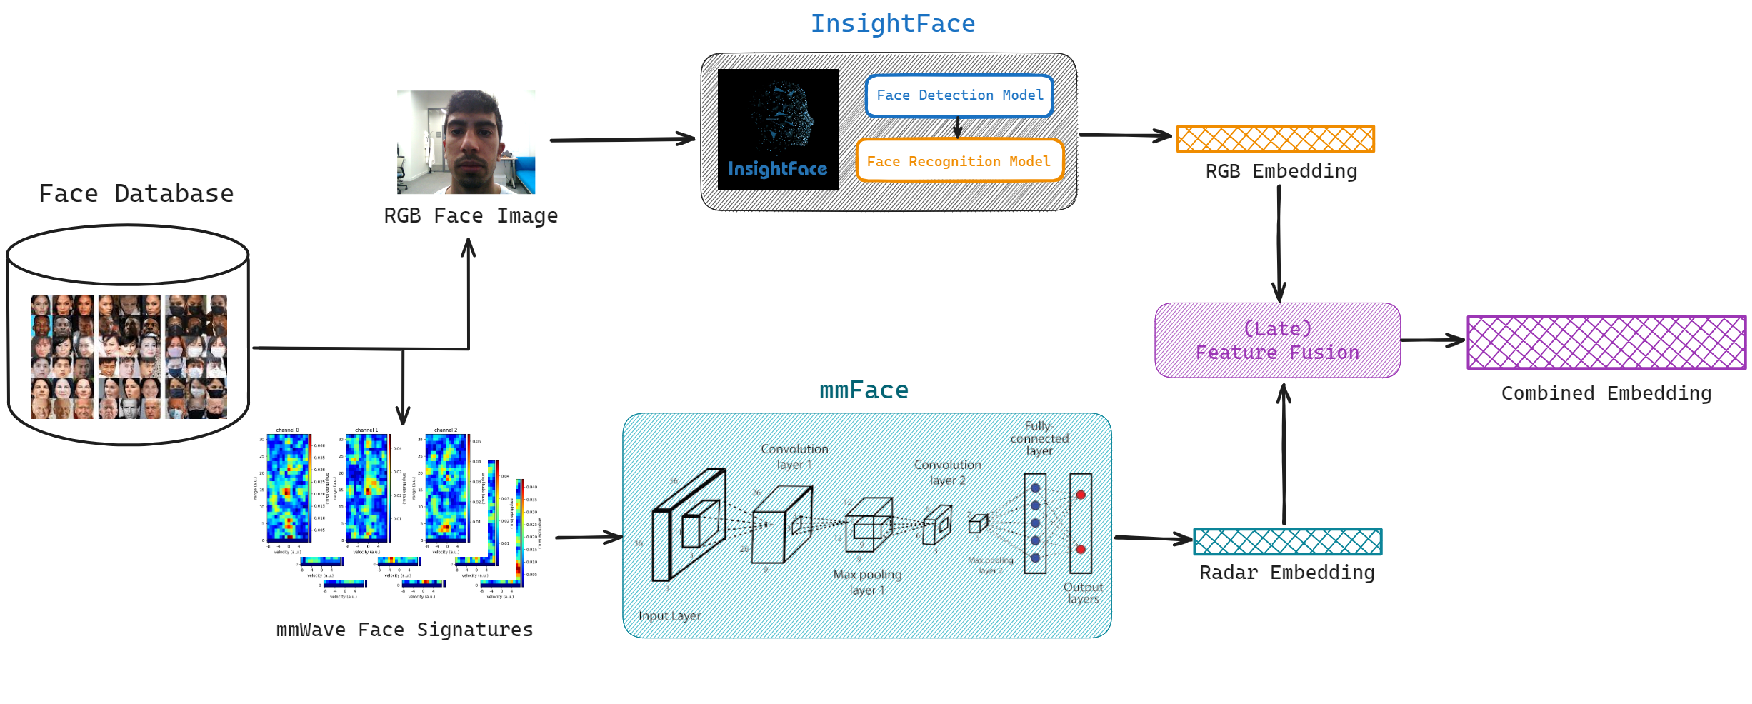
\includegraphics[width=1\textwidth]{images/model_architecture.pdf}
    \vspace{-1.1cm}
    \caption{High-level model architecture of our proposed system.}
    \vspace{-2cm}
    \label{fig:model_architecture}
\end{figure}

\newpage
Our proposed model, mmFace, will employ a CNN-based architecture, which is particularly effective for processing image-like data. The radar bursts obtained during the data collection phase will be transformed into Complex Range-Doppler (CRD) maps \cite{lien2016soli,hayashi2021radarnet} prior to feeding it into the model. Face scans will be collected using the Google Soli's short configuration which operates at a centre frequency of 60 GHz, with a maximum bandwidth $B$ of 5.5 GHz, and bursts sampled at 25 Hz. This gives a range resolution of $\frac{c}{2B} = 2.7$ cm, where $c$ denotes the speed of light. Given that Intel RealSense captures RGB-D frames at a different sampling rate of 30 frames per second (FPS), timestamp information is also recorded for the possibility of synchronising the two modalities for early data fusion.

As explained before, the data fusion techniques we plan to investigate include late, feature-level fusion and late, decision-level fusion. Pure intermediate fusion is not feasible due to the black-box treatment of the InsightFace model making it difficult to integrate information from both modalities within its hidden layers. Nonetheless, late, feature-level fusion remains viable, combining the outputs of the final layers of each model to form an embedding containing both the RGB and radar features. Similarly, decision-level fusion will be explored since this entails mixing the predictions from the individual models. Early fusion presents significant challenges due to the dissimilarities in sampling rates and data formats of the two modalities. The CRD maps must be synchronised and transformed into a depth image-like format before merging with the RGB images. Furthermore, this would require a whole new training cycle with the mmFace model which may be infeasible within the project's timeframe. However, should time permit, we will consider investigating this approach.

We plan to adopt a ResNet-based architecture for mmFace due to its refinements over its predecessors like AlexNet \cite{krizhevsky2012imagenet} and VGGNet \cite{simonyan2014very}. The ResNet framework \cite{he2016deep} incorporates "skip connections" and residual blocks to resolve the vanishing gradient problem encountered in VGGNet, allowing scaling of the network beyond the 19-layer limitation. This support for deeper networks provides a strong foundation for the mmFace model for learning the complex radar face signatures.

The dataset, comprising 50 participants, will be divided by subjects into an $80\%/10\%/10\%$ split for training, validation, and testing. Given the dataset's small size, a larger proportion is allocated for training to ensure the model can learn effectively. Following training, the testing phase will evaluate the distinctiveness of the output face embeddings. For accurate classifications, each person's face must be spatially separable in the high-dimensional embedding space allowing for unambiguous identification. t-SNE visualisations \cite{van2008visualizing} will be employed to visually inspect and confirm this is the case by comparing against the original data. In addition, standard classification accuracies will be calculated to verify the model's identity recognition capabilities against randomly selected ground truths. This also allows benchmarking our results against previous studies on radar-based 3D facial recognition.


\subsection{Progress}
\label{approach:progress}
To date, progress in the project has been promising, bolstering confidence in its successful completion. The data acquisition phase has begun effectively, with the facial data of 18 participants having been captured following the plan laid out in Section \ref{approach:data_acquisition}. We aim to expedite this process throughout January in order to reach the target of 50 participants with increased advertisements. The feasibility of InsightFace has also been validated through an experiment involving the recognition of famous NBA basketball players. The model, trained on a variety of images sourced from the web, demonstrated a high accuracy of 98.2\%. All work is being implemented in Python due to its extensive suite of powerful libraries useful for machine learning such as NumPy \cite{harris2020array} and PyTorch \cite{paszke2019pytorch}. 

To illustrate the data acquisition process used thus far, data samples of a single subject are provided in the left half of Figure \ref{fig:rgb_crd_plot}. This grid shows RGB frames recorded from all 15 scenarios, with the three different conditions along the rows and the five pose variations along the columns. For brevity, the conditions are abbreviated as outlined in Table \ref{tab:conditions}.

\begin{table}[h!]
    \centering
    \resizebox{0.49\textwidth}{!}{
        \begin{tabular}{|c|c|c|}
            \hline
            \textbf{Abbreviation} & \textbf{Expanded Forms}\\
            \hline
            \hline
            NO & No Occlusion \\
            \hline
            O & Occlusion \\
            \hline
            RLC & Regular Lighting Condition \\
            \hline
            DLC & Dim Lighting Condition \\
            \hline
        \end{tabular}
    }
    \caption{Table displaying full forms for abbreviations describing experiment conditions.}
    \label{tab:conditions}
\end{table}

Work has also been conducted in converting the data collected from our acquisition experiments into formats suitable for our proposed model. We have successfully transformed the radar bursts into CRD maps, which can be plotted displaying intensities of received waves into discrete Doppler bins along the $x$-axis and Range bins along the $y$-axis. A data sample of a single CRD frame can be observed in the right half of Figure \ref{fig:rgb_crd_plot}.

\begin{figure}[H]
    \centering
    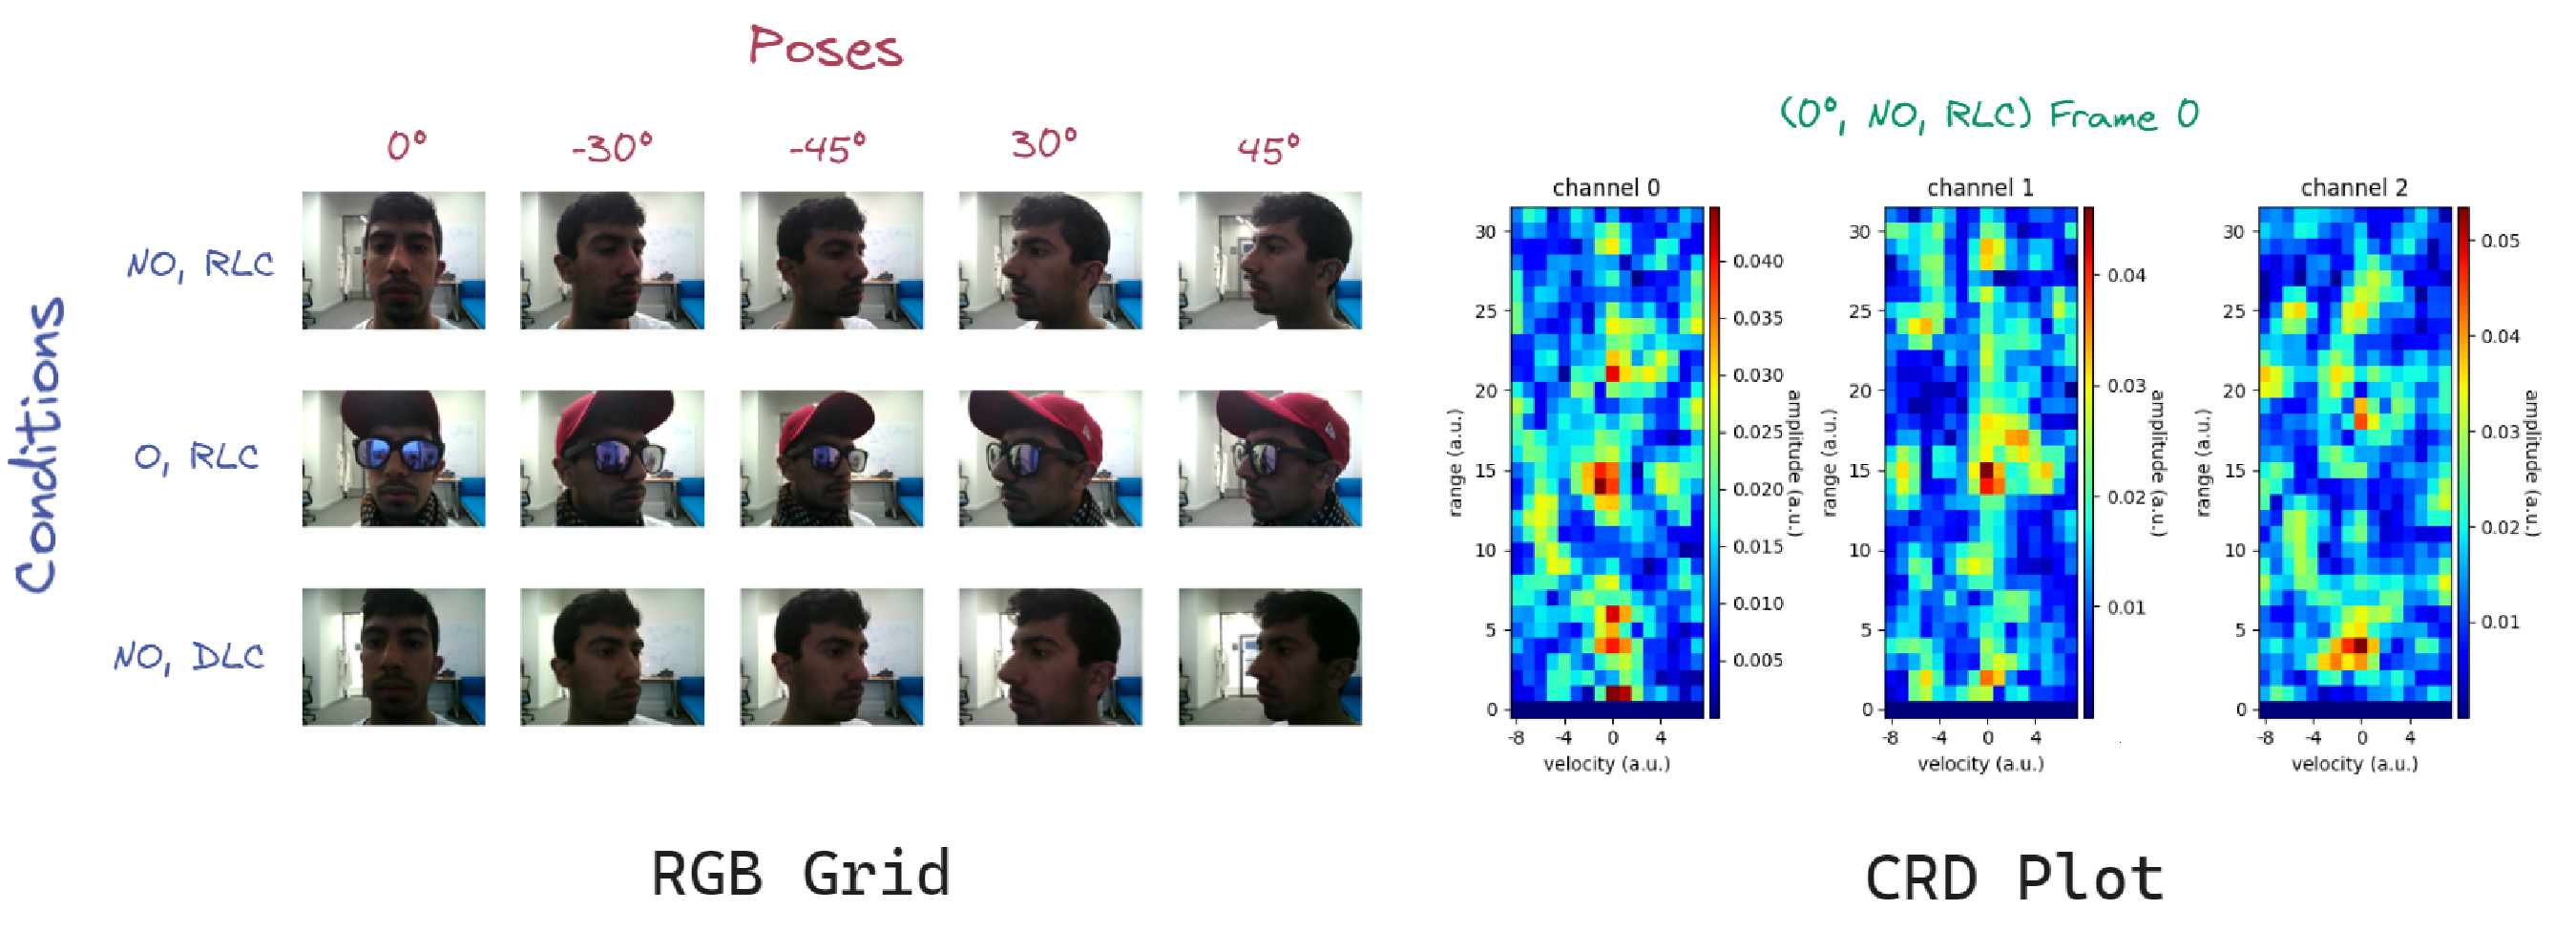
\includegraphics[width=0.99\textwidth]{images/CRD_RGB_plot.pdf}
    \caption{Data samples collected for Subject 0. The left figure shows the RGB frames of all 15 scenarios organised by pose and condition. The right figure plots a single CRD frame showing amplitudes of reflected waves detected by the three receiving channels of the Soli categorised into discrete Range-Doppler bins}
    \label{fig:rgb_crd_plot}
\end{figure}


%%%%%%%%%%%%%%%%%%%%%%%%%%%%%%%%%%%%%%%%%%%%%%%%%%%%%%%%%%%%%%%%%%%
\section{Work Plan}
% show how you plan to organize your work, identifying intermediate deliverables and dates.
Given that the project delves into the relatively new field of mmWave-based applications, a large amount of prerequisite knowledge is necessary before devising a solution to the problem of 3D face recognition. This research process will continue throughout the remaining duration of the project since there are still many hurdles to overcome. 

In order to alleviate the effects of these hurdles, it is important to look ahead and postulate the main problems that can occur by delineating a thorough plan of the next steps. As stated in the Progress Section \ref{approach:progress}, the data acquisition process is planned to be accelerated in January to gather the remaining 32 participants needed to reach our goal. Simultaneously, it is possible to implement and experiment with different configurations of our proposed mmFace CNN, aiming to identify the most effective setup for learning from the CRD data format. This provides a sufficient amount of time to train, validate, and test our model with the decently sized dataset we will collect. In addition, multiple models will be trained with varying degrees of missing CRD frames to assess the minimum amount of radar data required to still yield high recognition rates.

An evaluation stage will follow, involving t-SNE visualisations and classification experiments in order to empirically gauge the final models' performances, trained with differing amounts of the data. The calculated accuracy metrics will also be compared against the results from previous mmWave-based face recognition models, specifically examining the impact of integrating RGB information. The work plan delineated here can be visualised in Figure \ref{fig:gantt_chart} in the form of a Gantt chart.

\begin{figure}[h!]
    \centering
    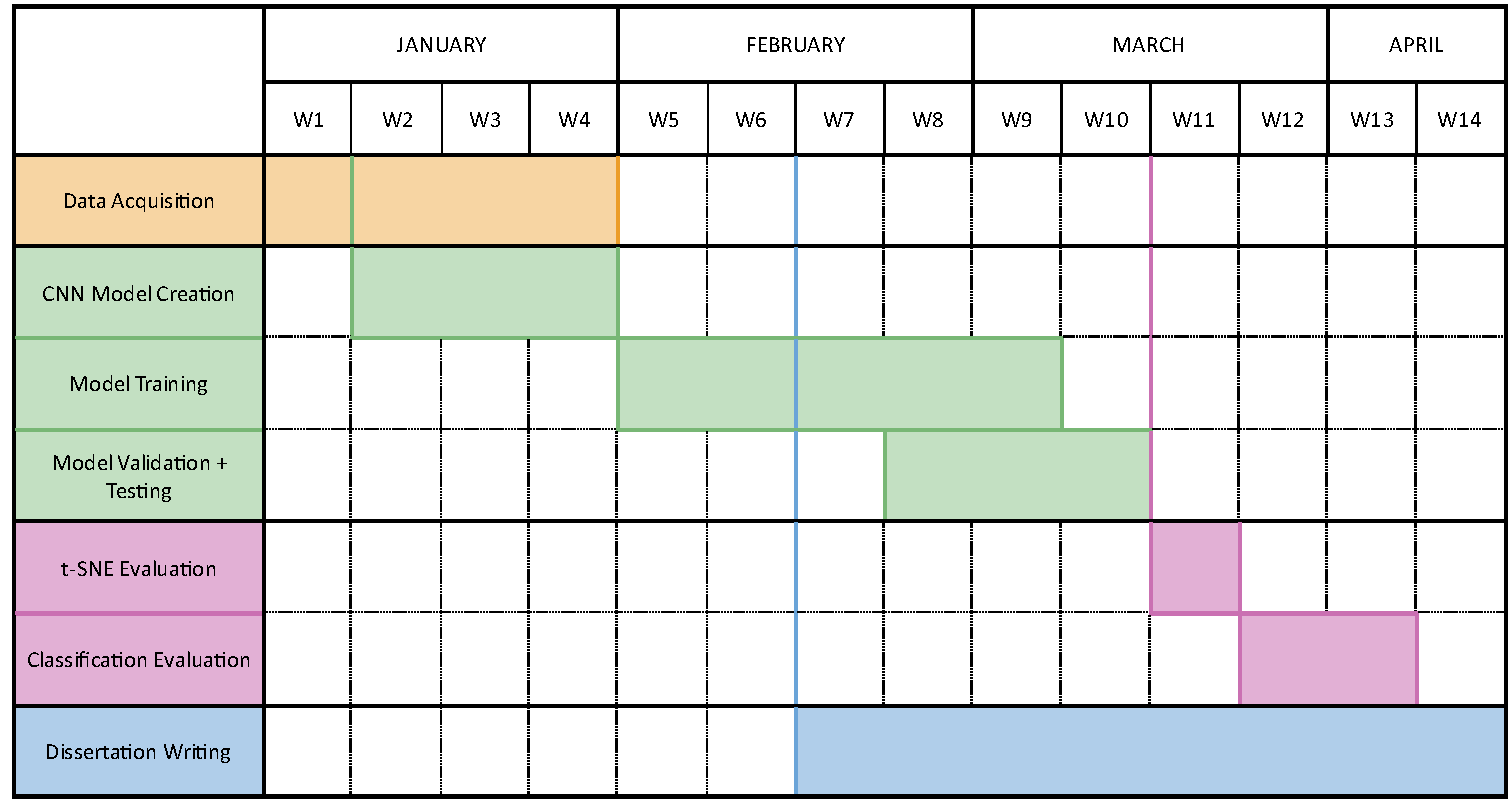
\includegraphics[width=1\textwidth]{images/gantt_chart.pdf}
    \caption{Gantt Chart showing the work plan for the next few months.}
    \label{fig:gantt_chart}
\end{figure}


%%%%%%%%%%%%%%%%%%%%%%%%%%%%%%%%%%%%%%%%%%%%%%%%%%%%%%%%%%%%%%%%%%%
% it is fine to change the bibliography style if you want
\bibliographystyle{unsrt}
\bibliography{interim}
\end{document}
